%%%%%%%%%%%%%%%%%%%%%%%%%%ch4-4
\begin{frame}[shrink]
  \frametitle{ch4.信号波形的检测}
  \framesubtitle{ch4-3. 一般二元信号波形的检测---正交级数展开法}
  \tableofcontents[hideallsubsections]
\end{frame}

\section{一般二元信号波形的检测---正交级数展开法}

\begin{frame}{一般二元信号波形的检测---信号模型}
在简单二元信号的波形检测中,假设$H_0$下和假设$H_1$的接收信号分别为:
\begin{align*}
&H_0: x(t)=s_0(t)+n(t), &&0\le t\le T\\
&H_1: x(t)=s_(t)+n(t), &&0\le t\le T
\end{align*}
其中, $s_0(t)$是能量为$E_0$的确知信号, $s_1(t)$是能量为$E_1$的确知信号
$n(t)$是均值为零, 功率谱密度为$N_0/2$的\textbf{高斯白噪声}。
\end{frame}

\begin{frame}[shrink]{接收信号MATLAB仿真$H_1$}
$H_1: x(t)=5\sin(t)+n(t),\quad 0 \le t\le 2\pi $\\
\vspace{0.5cm}
\begin{columns}%[T]
\column{0.05\textwidth}
~\\
\vspace{0.5cm}
$s_1(t)$\\
\vspace{0.7cm}
$n(t)$\\
\vspace{0.7cm}
$x(t)$
\column{0.95\textwidth}
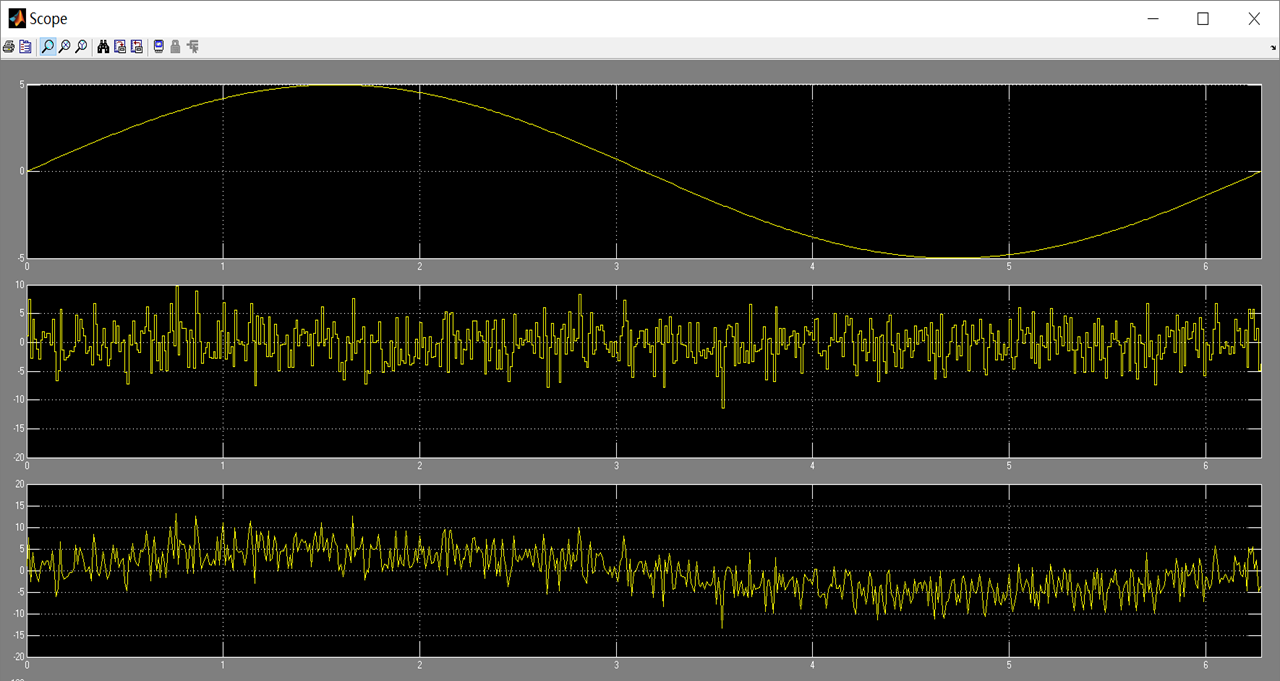
\includegraphics[scale=0.5]{matlab2-1}
\end{columns}
\end{frame}

\begin{frame}[shrink]{接收信号MATLAB仿真$H_0$}
$H_0: x(t)=5\sin(2t)+n(t),\quad 0 \le t\le 2\pi $\\
\vspace{1.8cm}
\begin{columns}%[t]
	\column{0.05\textwidth}
	~\\
	%\vspace{1cm}
	$s_0(t)$\\
	\vspace{1cm}
	$n(t)$\\
	\vspace{1.5cm}
	$x(t)$
	\column{0.95\textwidth}
	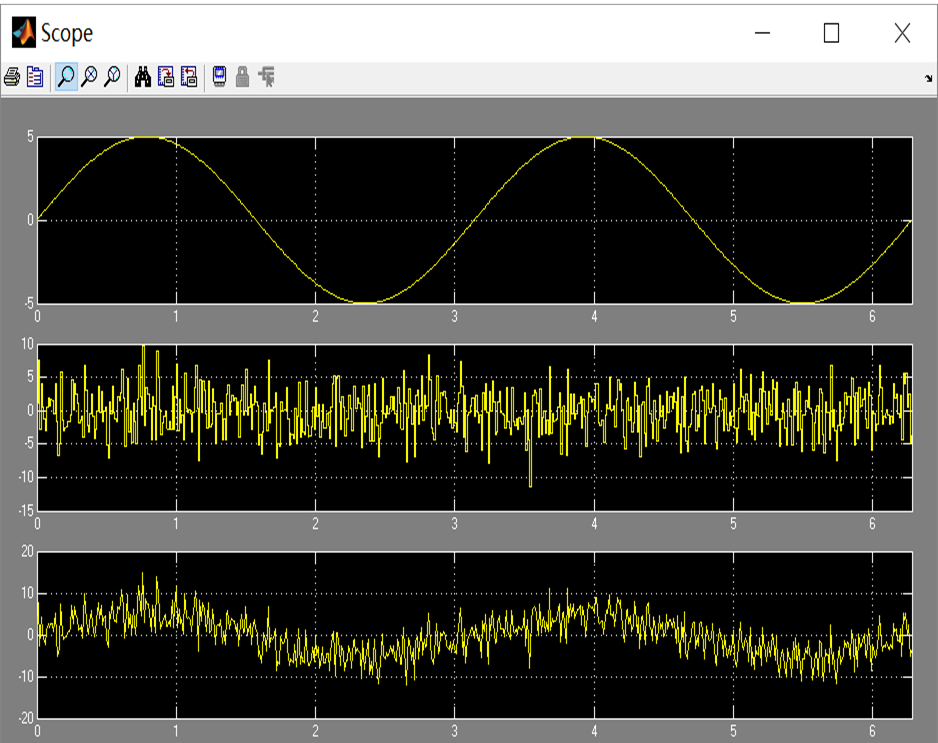
\includegraphics[scale=0.4]{matlab2-2}
\end{columns}
\end{frame}

\begin{frame}{检测步骤}
\begin{enumerate}
	\setlength{\itemsep}{.5cm}
	\item 首先,利用随机过程的正交级数展开,将随机过程用一组随机变量来表示;
	\item 然后,针对展开得到的随机变量,利用第三章的统计检测方法,构建贝叶斯检测表达式;
	\item 最后,令N趋向于无穷大, 利用展开系数与随机过程之间的表示关系,构建波形信号的检测表达式。
\end{enumerate}
\begin{block}{Notes}
	\begin{itemize}
		\item 确知信号的正交级数展开的展开系数是一组确定的值。
		\item 随机过程的正交级数展开的展开系数是一组随机变量,卡亨南-洛维
		展开可保证展开系数之间不相关。
	\end{itemize}
\end{block}
\end{frame}

\begin{frame}{判决表达式---步骤1}
$H_0: x(t)=s_0(t)+n(t),\quad 0\le t\le T$\\
$H_1: x(t)=s_1(t)+n(t),\quad 0\le t\le T$\\
\textbf{\textcolor{blue}{步骤1,选一组完备的正交函数集$\{f_k(t),k=1,2,\cdots \}$, 对接收信号进行正交级数展开,得到一组随机变量$x_k$}}\\
因为信号$s_0(t)$和$s_1(t)$是确知信号, $n(t)$是均值为0的高斯白噪声,所以可以任选正交函数集$\{f_k(t)\}$
\begin{align*}
&x(t)=\lim\limits_{N\to\infty}^N\sum\limits_{k=1}^Nx_kf_k(t)&&x_k=\int_{0}^{T}x(t)f_k(t)dt \\
&H_0: x_k=s_{0k}+n_k,k=1,2,\dots &&n_k=\int_{0}^{T}n(t)f_k(t)dt\\
&H_1: x_k=s_{1k}+n_k,k=1,2,\dots &&s_{ik}=\int_{0}^{T}s_i(t)f_k(t)dt, \quad i=0,1
\end{align*}
\end{frame}

\begin{frame}[shrink]{判决表达式---步骤1}
\begin{align*}
&x(t)=\lim\limits_{N\to\infty}^N\sum\limits_{k=1}^Nx_kf_k(t)&&x_k=\int_{0}^{T}x(t)f_k(t)dt \\
&H_0: x_k=s_{0k}+n_k,k=1,2,\dots &&n_k=\int_{0}^{T}n(t)f_k(t)dt\\
&H_1: x_k=s_{1k}+n_k,k=1,2,\dots &&s_{ik}=\int_{0}^{T}s_i(t)f_k(t)dt, \quad i=0,1
\end{align*}
\begin{itemize}
\item 信号$s_0(t)$和$s_1(t)$是确知信号, $n(t)$是均值为0,功率谱密度为$P_n(\omega)=N_0/2$的高斯白噪声;
\item 无论在假设$H_1$下还是在假设$H_2$下,接收信号的$x(t)$都是高斯随机过程;
\item 展开系数$x_k$是高斯随机过程的积分结果,因而$x_k$是高斯随机变量;
\item 展开系数$x_k$之间是互不相关的,也是相互统计独立的;
\item 高斯随机变量由均值和方差决定。由此求出两个假设下的概率密度函数$p(x_k|H_j),k=1,2,\dots;j=0,1$。
\end{itemize}
\end{frame}

\begin{frame}[shrink]{判决表达式---步骤1: 假设$H_0$下$x_k$的均值和方差}
\begin{align*}
&H_0: x_k=s_{0k}+n_k, \quad n_k=\int_{0}^{T}n(t)f_k(t)dt, \quad\text{由于$n(t)$是均值为零的高斯白噪声, }\\
&E[n(t)]=0, E[n(t)n(u)]=r_n(t-u) =\frac{N_0}{2}\delta(t-u)=\frac{N_0}{2},(\delta(t-u)=1,t=u)\\
&\text{$f_k(t)$是一组正交函数集, } \int_{0}^{T}f_j(t)f_k(t)dt=1,(j=k)
\end{align*}
\begin{align*}
E[x_k|H_0]&=E\left[\int_{0}^{T}x(t)f_k(t)dt\right]=E\left[\int_{0}^{T}(s_0(t)+n(t))f_k(t)dt\right]\\
&=E\left[\int_{0}^{T}s_0(t)f_k(t)dt\right]+\int_{0}^{T}E[n(t)]f_k(t)dt=s_{0k}\quad (\text{by }s_{0k}=\int_{0}^{T}s_0(t)f_k(t)dt)\\
Var[x_k|H_0]&=E[(x_k-E[x_k])^2]=E[n_k^2]=E\left[\int_{0}^{T}n(t)f_k(t)dt\int_{0}^{T}n(u)f_k(u)du\right]\\
&=\int_{0}^{T}f_k(t)\left\{\int_{0}^{T}E[n(t)n(u)]f_k(u)du\right\}dt=\int_{0}^{T}f_k(t)\left[\int_{0}^{T}\frac{N_0}{2}\delta(t-u)f_k(u)du\right]dt\\
&=\int_{0}^{T}f_k(t)\frac{N_0}{2}f_k(t)dt=\frac{N_0}{2}
\end{align*}
\end{frame}

\begin{frame}[shrink]{判决表达式---步骤1: 假设$H_1$下$x_k$的均值和方差}
\begin{align*}
H_1: x_k=s_{1k}+n_k, \quad s_{1k}=\int_{0}^{T}s_1(t)f_k(t)dt, \quad n_k=\int_{0}^{T}n(t)f_k(t)dt
\end{align*}
\begin{align*}
E[x_k|H_1]&=E[s_{1k}+n_k]&\text{by }x_k=s_{1k}+n_k \\
&=E(s_{1k})+E(n_k)&\text{by }E(n_k)=0 \\
&=E(s_{1k})=s_{1k}&\text{(确知信号展开系数为确定量,其均值就是本身)}\\
Var[x_k|H_1]&=E[(x_k-E[x_k])^2]&\text{by }x_k=s_{1k}+n_k,E[x_k]=s_{1k}\\
&=E[(s_{1k}+n_k-s_{1k})^2]&\\
&=E[n_k^2]=\frac{N_0}{2}&
\end{align*}
\end{frame}

\begin{frame}[shrink]{判决表达式---步骤1: 假设$H_0,H_1$下$x_k$的概率密度}
\begin{align*}
E[x_k|H_0]=s_{0k},   &\quad Var[x_k|H_1]=\frac{N_0}{2}\\
E[x_k|H_1]=s_{1k}, &\quad Var[x_k|H_1]=\frac{N_0}{2}
\end{align*}
\begin{align*}
p(x_k|H_0)&=\left(\frac{1}{\pi N_0}\right)^{1/2}\exp\left(-\frac{(x_k-s_{0k})^2}{N_0}\right), k=1,2,\cdots\\
p(x_k|H_1)&=\left(\frac{1}{\pi N_0}\right)^{1/2}\exp\left(-\frac{(x_k^2-s_{1k})^2}{N_0}\right), k=1,2,\cdots
\end{align*}
\end{frame}

\begin{frame}[shrink]{判决表达式---步骤2: 假设$H_0,H_1$下$\bm{x}_N$的概率密度}
\textbf{\textcolor{blue}{步骤2,利用前$N$项展开系数, 构建似然比检验。由于信道是加性高斯白噪声, 由卡亨南---洛维展开可知, 各展开系数是不相关的, 因而也是相互独立的。}}
\begin{align*}
&p(\bm{x}_N|H_0)=\prod_{k=1}^{N}p(x_k|H_0)=\prod_{k=1}^{N}\left(\frac{1}{\pi N_0}\right)^{1/2}\exp\left(-\frac{(x_k-s_{0k})^2}{N_0}\right)\\
&p(\bm{x}_N|H_1)=\prod_{k=1}^{N}p(x_k|H_1)=\prod_{k=1}^{N}\left(\frac{1}{\pi N_0}\right)^{1/2}\exp\left(-\frac{(x_k-s_{1k})^2}{N_0}\right)\\
&\bm{x}_N=(x_1,x_2,\cdots)^T
\end{align*}	
\end{frame}

\begin{frame}[shrink]{判决表达式---步骤2: 似然比}
\begin{align*}
\lambda(\bm{x}_N)=\frac{p(\bm{x}_N|H_1)}{p(\bm{x}_N|H_0)}&\mathop{\gtrless}_{H_0}^{H_1}\eta\\
\frac{\prod\limits_{k=1}^{N}\left(\frac{1}{\pi N_0}\right)^{1/2}\exp\left(-\frac{(x_k-s_{1k})^2}{N_0}\right)}
{\prod\limits_{k=1}^{N}\left(\frac{1}{\pi N_0}\right)^{1/2}\exp\left(-\frac{(x_k-s_{0k})^2}{N_0}\right)}&\mathop{\gtrless}_{H_0}^{H_1}\eta
\end{align*}
化简,得到
\[\ln\lambda(\bm{x}_N)=\frac{p(\bm{x}_N|H_1)}{p(\bm{x}_N|H_0)}=\frac{2}{N_0}\sum\limits_{k=1}^{N}x_ks_{1k}-\frac{2}{N_0}\sum\limits_{k=1}^{N}x_ks_{0k}+\frac{1}{N_0}\sum\limits_{k=1}^{N}s_{0k}^2-\frac{1}{N_0}\sum\limits_{k=1}^{N}s_{1k}^2\mathop{\gtrless}_{H_0}^{H_1}\ln\eta \]
\end{frame}

\begin{frame}[shrink]{判决表达式---步骤3: 将离散判决式变成连续形式}
\[\ln\lambda(\bm{x}_N)=\frac{p(\bm{x}_N|H_1)}{p(\bm{x}_N|H_0)}=\frac{2}{N_0}\sum\limits_{k=1}^{N}x_ks_{1k}-\frac{2}{N_0}\sum\limits_{k=1}^{N}x_ks_{0k}+\frac{1}{N_0}\sum\limits_{k=1}^{N}s_{0k}^2-\frac{1}{N_0}\sum\limits_{k=1}^{N}s_{1k}^2\mathop{\gtrless}_{H_0}^{H_1}\ln\eta \]
\textbf{\textcolor{blue}{步骤3, 令$N\to\infty$, 将离散判决式变成连续形式}}
因为在两个假设下接收信号$x(t)(0\le t\le T)$的展开系数$x_k(k=1,2,\cdots)$是无穷多个,而离散形式判决式只是取前有限$N$项的结果,因此应对上式取$N\to\infty$的极限。
\begin{align*}
\ln\lambda(x(t))&\mathop{=}^{def}\lim\limits_{N\to\infty}[\ln\lambda(\bm{x}_N)]\qquad\text{(推导见简单二元信号波形检测)}\\
&=\lim\limits_{N\to\infty}\left(\frac{2}{N_0}\sum\limits_{k=1}^{N}x_ks_{1k}-\frac{2}{N_0}\sum\limits_{k=1}^{N}x_ks_{0k}+\frac{1}{N_0}\sum\limits_{k=1}^{N}s_{0k}^2-\frac{1}{N_0}\sum\limits_{k=1}^{N}s_{1k}^2\right)\\
&=\frac{2}{N_0}\int_{0}^{T}x(t)s_1(t)dt-\frac{2}{N_0}\int_{0}^{T}x(t)s_0(t)dt+\frac{E_0}{N_0}-\frac{E_1}{N_0}\\
l[x(t)]&\mathop{=}^{def}\int_{0}^{T}x(t)s_1(t)dt-\int_{0}^{T}x(t)s_0(t)dt\mathop{\gtrless}_{H_0}^{H_1}\frac{N_0}{2}\ln\eta+\frac{E_1}{2}-\frac{E_0}{2}\mathop{=}^{def}\gamma
\end{align*}
\end{frame}

\begin{frame}{一般二元信号波形的检测---检测系统结构}
\[l[x(t)]\mathop{=}^{def}\int_{0}^{T}x(t)s_1(t)dt-\int_{0}^{T}x(t)s_0(t)dt\mathop{\gtrless}_{H_0}^{H_1}\frac{N_0}{2}\ln\eta+\frac{E_1}{2}-\frac{E_0}{2}\mathop{=}^{def}\gamma \]
~\\
\centering
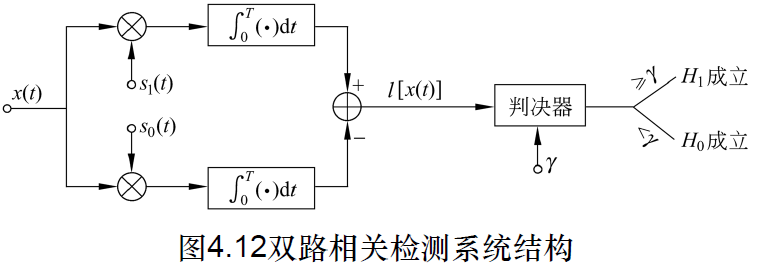
\includegraphics[scale=0.45]{4-12}\\
\leftline{检测统计量$l[x(t)]$由接收信号$x(t)$与确知信号$s_0(t)$和$s_1(t)$经相关运算得到。}
\leftline{由互相关器和判决器实现。}
\end{frame}

\begin{frame}{检测系统MATLAB仿真}
$H_0: x(t)=5\sin(t)+n(t),\quad 0 \le t\le 2\pi $\\
$H_1: x(t)=5\sin(2t)+n(t),\quad 0 \le t\le 2\pi $\\
~\\
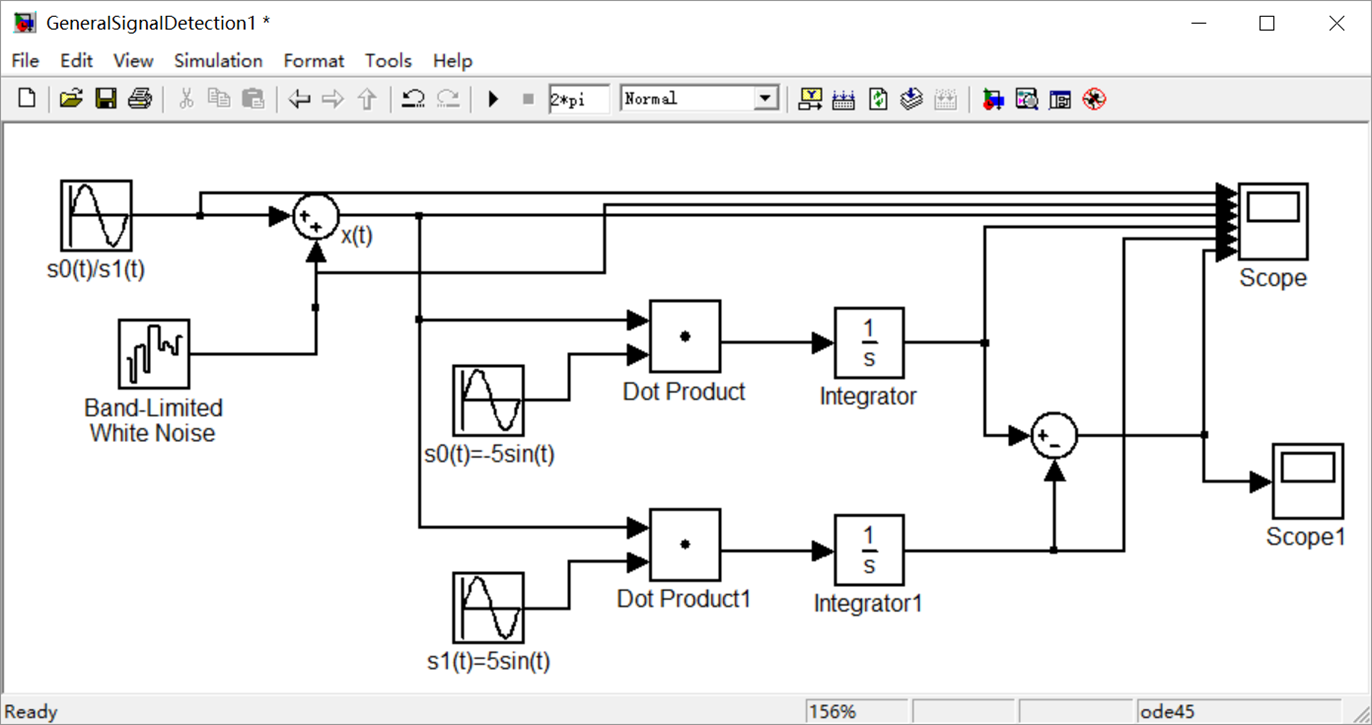
\includegraphics[scale=0.45]{matlab2-3}
\end{frame}

\begin{frame}[shrink]{接收信号MATLAB仿真$H_1$}
$H_1: x(t)=5\sin(t)+n(t),\quad 0 \le t\le 2\pi $\\
\vspace{0.5cm}
\begin{columns}[T]
	\column{0.15\textwidth}
	\vspace{0.6cm}
	$5\sin(t)$\\
	\vspace{0.4cm}
	$n(t)$\\
	\vspace{0.4cm}
	$x(t)$\\
	\vspace{0.4cm}
	$\int_{0}^{T}x(t)s_1(t)dt$\\
	\vspace{0.4cm}
	$\int_{0}^{T}x(t)s_0(t)dt$\\
	\vspace{0.4cm}
	$l(x(t)]$\\
	\column{0.8\textwidth}
	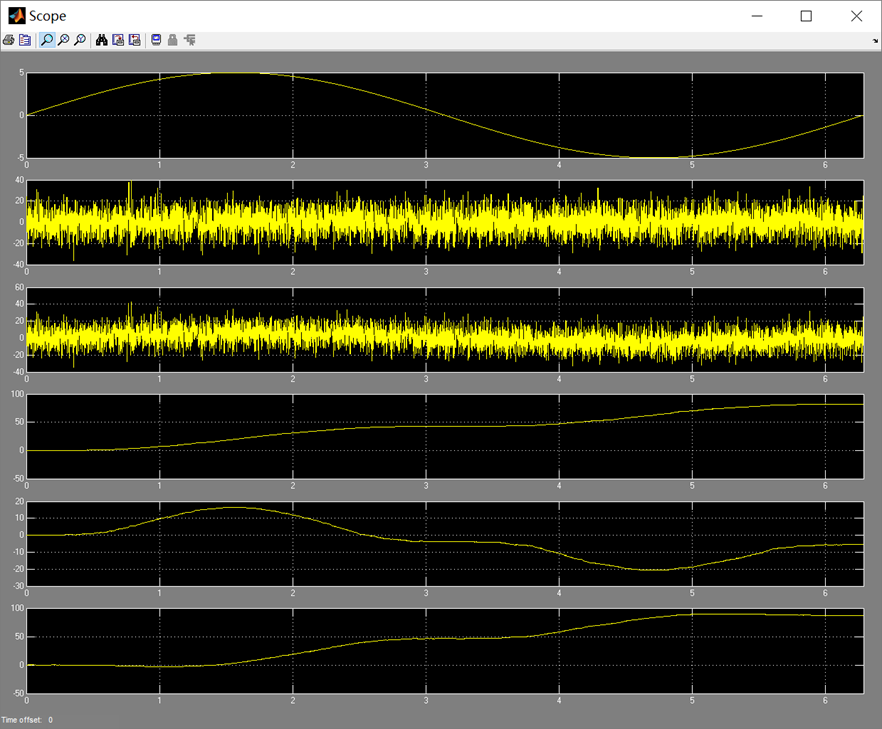
\includegraphics[scale=0.5]{matlab2-4}
\end{columns}
\vspace{0.2cm}
\end{frame}

\begin{frame}[shrink]{接收信号MATLAB仿真$H_0$}
$H_0: x(t)=5\sin(2t)+n(t),\quad 0 \le t\le 2\pi $\\
\vspace{0.5cm}
\begin{columns}[T]
	\column{0.15\textwidth}
	\vspace{0.6cm}
	$5\sin(2t)$\\
	\vspace{0.4cm}
	$n(t)$\\
	\vspace{0.4cm}
	$x(t)$\\
	\vspace{0.4cm}
	$\int_{0}^{T}x(t)s_1(t)dt$\\
	\vspace{0.4cm}
	$\int_{0}^{T}x(t)s_0(t)dt$\\
	\vspace{0.4cm}
	$l(x(t)]$\\
	\column{0.8\textwidth}
	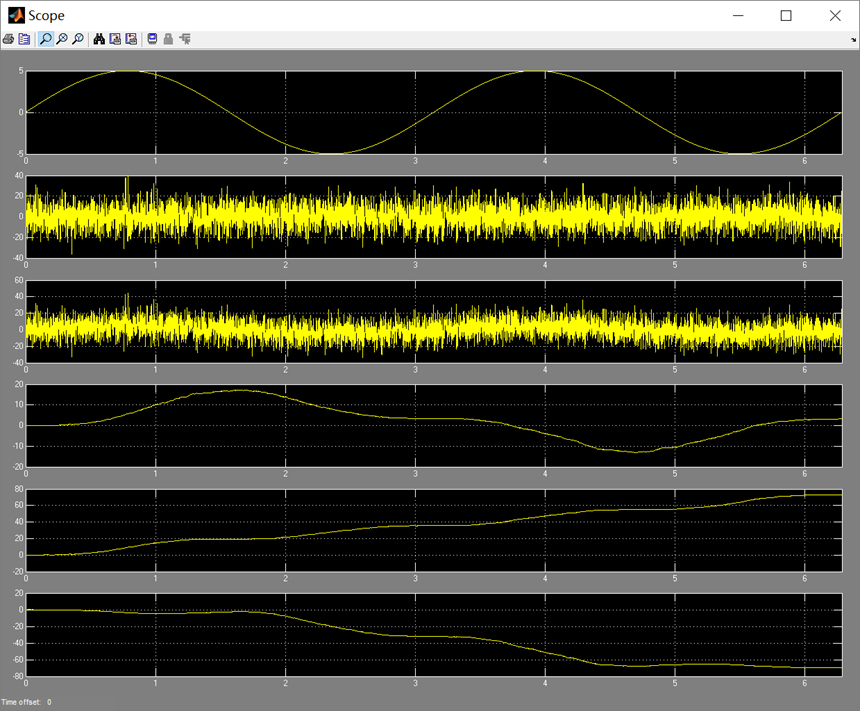
\includegraphics[scale=0.5]{matlab2-5}
\end{columns}
\vspace{0.2cm}
\end{frame}

\begin{frame}{一般二元信号波形检测---步骤归纳}
\begin{enumerate}
	\setlength{\itemsep}{.5cm}
	\item 首先,利用随机过程的正交级数展开,将随机过程用一组随机变量来表示;
	\item 然后,针对展开得到的随机变量,利用第三章的统计检测方法,构建贝叶斯检测表达式;
	\item 最后,令N趋向于无穷大, 利用展开系数与随机过程之间的表示关系,构建波形信号的检测表达式。
\end{enumerate}
\[l[x(t)]\mathop{=}^{def}\int_{0}^{T}x(t)s_1(t)dt-\int_{0}^{T}x(t)s_0(t)dt\mathop{\gtrless}_{H_0}^{H_1}\frac{N_0}{2}\ln\eta+\frac{E_1}{2}-\frac{E_0}{2}\mathop{=}^{def}\gamma \]
\end{frame}

\section{检测系统性能分析}

\begin{frame}{检测系统性能分析}
\[l[x(t)]\mathop{=}^{def}\int_{0}^{T}x(t)s_1(t)dt-\int_{0}^{T}x(t)s_0(t)dt\mathop{\gtrless}_{H_0}^{H_1}\frac{N_0}{2}\ln\eta+\frac{E_1}{2}-\frac{E_0}{2}\mathop{=}^{def}\gamma \]
\textbf{统计量}
\[l[x(t)]\mathop{=}^{def}\int_{0}^{T}x(t)s_1(t)dt-\int_{0}^{T}x(t)s_0(t)dt\]
\textbf{两个判决概率}
\[P(H_1|H_0)=\int_{\gamma}^{\infty}p(l|H_0)dl\quad P(H_1|H_1)=\int_{\gamma}^{\infty}p(l|H_1)dl \]
\textbf{\textcolor{blue}{由于接收信号$x(t)$是以高斯随机过程,所以统计量$l$为服从高斯分布的随机变量。}}
\end{frame}

\begin{frame}{检测系统性能分析}
\textbf{统计量}
\[l[x(t)]\mathop{=}^{def}\int_{0}^{T}x(t)s_1(t)dt-\int_{0}^{T}x(t)s_0(t)dt\]
\textbf{假设$H_0$下, $l$的均值和方差为}
\begin{align*}
E[l|H_0]&=E\left[\int_{0}^{T}x(t)s_1(t)dt|H_0-\int_{0}^{T}x(t)s_0(t)dt|H_0\right]=\rho\sqrt{E_1E_0}-E_0\\
Var[l|H_0]&=E\left\{\left[(l|H_0)-E[l|H_0]\right]^2\right\}=\frac{N_0}{2}(E_1+E_0-2\rho\sqrt{E_0E_1})
\end{align*}
式中, 信号$s_0(t)$和$s_1(t)$之间的波形相关系数$\rho$为 \[\rho\mathop{=}\limits^{def}\frac{1}{\sqrt{E_{0}E_{1}}}\int_{0}^{T}s_0(t)s_1(t)dt,\quad(|\rho|\le 1)\]
\end{frame}

\begin{frame}{检测系统性能分析}
\textbf{统计量}
\[l[x(t)]\mathop{=}^{def}\int_{0}^{T}x(t)s_1(t)dt-\int_{0}^{T}x(t)s_0(t)dt\]
\textbf{类似地, 假设$H_1$下, $l$的均值和方差为}
\begin{align*}
E[l|H_1]&=E_1-\rho\sqrt{E_1E_0}\\
Var[l|H_0]&=\frac{N_0}{2}(E_1+E_0-2\rho\sqrt{E_0E_1})
\end{align*}
式中, 信号$s_0(t)$和$s_1(t)$之间的波形相关系数$\rho$为 \[\rho\mathop{=}\limits^{def}\frac{1}{\sqrt{E_{0}E_{1}}}\int_{0}^{T}s_0(t)s_1(t)dt,\quad(|\rho|\le 1)\]
\end{frame}

\begin{frame}{检测系统性能分析}
定义偏移系数$d^2$为
\[d^2\mathop{=}\limits^{def}\frac{(E(l|H_1)-E(l|H_0))^2}{Var(l|H_0)}=\frac{2}{N_0}(E_1+E_0-2\rho\sqrt{E_0E_1}) \]
判决概率为
\begin{align*}
P(H_1|H_0)&=\int_{\gamma}^{\infty}p(l|H_0)dl=Q\left(\frac{\ln\eta}{d}+\frac{d}{2}\right)\\
P(H_1|H_1)&=\int_{\gamma}^{\infty}p(l|H_1)dl=Q\left(\frac{\ln\eta}{d}-\frac{d}{2}\right)\\
\end{align*}
\end{frame}

\section{最佳信号波形设计}

\begin{frame}[shrink]{最佳信号波形设计(1)}
偏移系数$d^2$和波形相关系数$\rho$:
\[d^2=\frac{2}{N_0}(E_1+E_0-2\rho\sqrt{E_0E_1}),\quad \rho=\frac{1}{\sqrt{E_{0}E_{1}}}\int_{0}^{T}s_0(t)s_1(t)dt,\quad(|\rho|\le 1) \]
因为$|\rho|\le 1$, 所以当$\rho=-1$时, $d^2$可取最大值。令$E_0$与$E_1$之和为常数, 则$E_0=E_1$时, $E_0E_1$最大。\\
所以, \textbf{\textcolor{blue}{在高斯白噪声条件下, 对于确知一般二元信号的波形检测, 当两个信号设计成互反信号时, 可在信号能量给定的约束下获得最好的检测性能, 而与信号的波形无关。}}
\begin{align*}
&\textbf{设}\quad E_0=E_1=E_s,\implies\sqrt{E_0E_1}=E_s\\
&\textbf{如果信号设计成$s_0(t)$和$s_1(t)$互反: }\quad s_0(t)=-s_1(t),\\
&\quad\int_{0}^{T}s_0(t)s_1(t)dt=E_s\implies |\rho|=-1\\
&d^2=\frac{8}{N_0}E_s\quad\textbf{取得最大值$\implies$最佳波形设计}
\end{align*}
\end{frame}

\begin{frame}{最佳信号波形设计(2)}
偏移系数$d^2$和波形相关系数$\rho$:
\[d^2=\frac{2}{N_0}(E_1+E_0-2\rho\sqrt{E_0E_1}),\quad \rho=\frac{1}{\sqrt{E_{0}E_{1}}}\int_{0}^{T}s_0(t)s_1(t)dt,\quad(|\rho|\le 1) \]
\textbf{设}$\quad E_0=E_1=E_s,\implies\sqrt{E_0E_1}=E_s$\\
\textbf{如果信号设计成$s_0(t)$和$s_1(t)$正交:}
 \begin{align*}
 &\int_{0}^{T}s_0(t)s_1(t)dt=0 \implies \rho=0 \\
 &d^2=\frac{4}{N_0}E_s
 \end{align*}
\textbf{检测性能差于信号互反时的波形设计}
\end{frame}

\begin{frame}{最佳信号波形设计(3)}
偏移系数$d^2$和波形相关系数$\rho$:
\[d^2=\frac{2}{N_0}(E_1+E_0-2\rho\sqrt{E_0E_1}),\quad \rho=\frac{1}{\sqrt{E_{0}E_{1}}}\int_{0}^{T}s_0(t)s_1(t)dt,\quad(|\rho|\le 1) \]
\textbf{设}$\quad E_0=E_1=E_s,\implies\sqrt{E_0E_1}=E_s$\\
\textbf{如果信号设计成:} 
\[0<\int_{0}^{T}s_0(t)s_1(t)dt\le E_s\implies 0<\rho\le 1 \]
\[\frac{4}{N_0}E_s>d^2\ge 0\]
$\rho\to 1, d^2\to 0$\textbf{检测性能}$\downarrow$, \textbf{信号波形设计不合理!}
\end{frame}

\begin{frame}{最佳信号波形设计}
\begin{block}{最佳波形设计$\rho=-1,s_0(t)=-s_1(t),d^2=\frac{8}{N_0}E_s,E_0=E_1=E_s$}
	在高斯白噪声条件下,对于确知一般二元信号的波形检测,当两个信号设计成互反信号时,可在信号能量给定的约束下获得最好的检测性能。
\end{block}
\begin{block}{$s_0(t),s_1(t)$正交波形设计$\rho=0,d^2=\frac{4}{N_0}E_s,E_0=E_1=E_s$}
	信号的检测性能差于同信号能量的反相信号。
\end{block}
\begin{block}{不合理波形设计$0<\rho\le 1,E_0=E_1=E_s$}
	$\frac{4}{N_0}E_s>d^2\ge 0\implies\rho\to 1,d^2\to 0$,检测性能逐步变差。
\end{block}
\end{frame}

\begin{frame}{检测步骤}
\begin{enumerate}
	\setlength{\itemsep}{.5cm}
	\item 首先,利用随机过程的正交级数展开,将随机过程用一组随机变量来表示;
	\item 然后,针对展开得到的随机变量,利用第三章的统计检测方法,构建贝叶斯检测表达式;
	\item 最后,令N趋向于无穷大, 利用展开系数与随机过程之间的表示关系,构建波形信号的检测表达式。
\end{enumerate}
\begin{block}{Notes}
	\begin{itemize}
		\item 确知信号的正交级数展开的展开系数是一组确定的值。
		\item 随机过程的正交级数展开的展开系数是一组随机变量,卡亨南-洛维
		展开可保证展开系数之间不相关。
	\end{itemize}
\end{block}
\end{frame}
